\section{What Governs the Loss: Order-Error and ACI's
Bound}

MinPredictedDegree matches by ascending predicted degree, so it depends
on the predictor \(\mu\) \emph{only through the order it induces on the
resources}. Two predictors that induce the same order produce identical
matchings; a monotone rescaling of \(\mu\) changes nothing. The natural
question is therefore not ``how large is the prediction error'' but
``which \emph{order} error governs the loss,'' and how tightly. This
section answers that empirically. It also requires care: the qualitative
fact that order --- not magnitude --- matters is \emph{already theorem}
in the literature, and we are explicit about what is prior and what is
ours.

\textbf{What is already known (ACI).} Aamand, Chen \& Indyk {[}ACI22,
Appendix D{]} prove, for MinPredictedDegree on the CLV-B model, that the
matching loss relative to the true expected degrees is at most
\(n - \mathrm{LIS}(p[\mu])\), where \(p[\mu]\) is the true weights
ordered by \(\mu\) and \(\mathrm{LIS}\) is the longest non-decreasing
subsequence --- a pure \emph{order} quantity. In particular a monotone
(order-preserving) predictor has \(p[\mu]\) already sorted, so
\(\mathrm{LIS}=n\), \(n-\mathrm{LIS}=0\), and the loss is zero. Thus
\emph{order-dependence} and \emph{the zero-effect of a monotone bias}
are ACI's results, not ours; our \texttt{systematic\_bias} error model
(a monotone rescale) has Kendall-\(\tau\equiv 0\) \emph{by construction}
and, consistently, leaves MPD's ratio exactly unchanged across the
benchmark (Section 3) --- an empirical confirmation of ACI's statement,
not a new finding.

Our contribution is to characterize \emph{how the bound behaves} and
\emph{which order measure predicts the realized loss}. We sweep the four
structured error models across strength and record, per model and level,
three quantities on the same instances: the actual MPD matching loss,
ACI's \(n-\mathrm{LIS}\), and the normalized Kendall-\(\tau\) order
error (\textbf{Figure 1}; \(n=1000\), Zipf exponent \(1.0\), 40 trials).

\begin{figure}
\centering
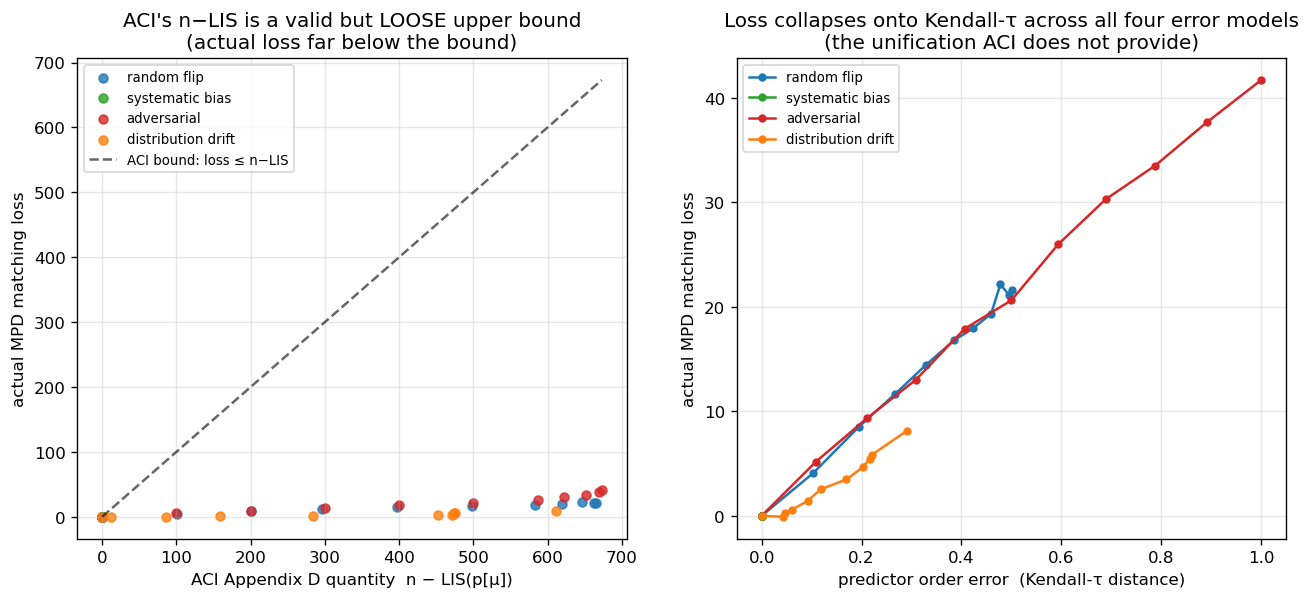
\includegraphics[width=1\linewidth,height=\textheight,keepaspectratio,alt={Order error, not magnitude, governs MPD's loss: (a) realized loss sits far below the n-\textbackslash mathrm\{LIS\} bound at every point; (b) the four error models collapse onto the Kendall-\textbackslash tau axis.}]{../../results/order_vs_theory.png}
\caption{Order error, not magnitude, governs MPD's loss: (a) realized
loss sits far below the \(n-\mathrm{LIS}\) bound at every point; (b) the
four error models collapse onto the Kendall-\(\tau\) axis.}
\end{figure}

\textbf{(i) ACI's \(n-\mathrm{LIS}\) bound is correct but very loose.}
The realized loss sits far below the \(n-\mathrm{LIS}\) upper bound at
every point --- by roughly \(16\times\) (adversarial) to \(75\times\)
(distribution-drift). Figure 1(a) plots loss against \(n-\mathrm{LIS}\)
with the \(y=x\) bound; all points lie close to the axis.

\textbf{(ii) \(n-\mathrm{LIS}\) saturates and cannot distinguish error
structures.} For every non-trivial error the quantity is pinned near its
maximum (\(n-\mathrm{LIS}\approx 610\)--\(673\) for \(n=1000\)), even
though the true losses differ by a factor of five across models ---
\(8.1\) (drift), \(21.6\) (random-flip), and \(41.7\) (adversarial) at
full strength. As an upper bound that is (almost) always \(\approx n\),
it carries little information about which prediction is actually more
harmful.

\textbf{(iii) Kendall-\(\tau\) is the governing order measure, and the
error models collapse onto it.} Plotting the realized loss against the
Kendall-\(\tau\) order error (Figure 1(b)), the four structured error
models fall on a single increasing curve: loss rises monotonically with
Kendall-\(\tau\) (\(0.29\to0.50\to1.0\) for drift, random-flip,
adversarial, tracking \(8.1\to21.6\to41.7\) in loss), with
\texttt{systematic\_bias} pinned at \(\tau=0\) and zero loss. The
quantity that \emph{predicts} the loss --- and unifies the error models
--- is the Kendall-\(\tau\) order distance, which \(n-\mathrm{LIS}\)
(saturated) cannot resolve.

\textbf{Takeaway (and scope).} We do not claim that order, rather than
magnitude, governs MPD --- ACI's Appendix D establishes that, and the
zero-effect of a monotone bias with it. What we add is a precise
empirical characterization: ACI's \(n-\mathrm{LIS}\) bound is loose by
one to nearly two orders of magnitude and saturates, whereas
Kendall-\(\tau\) predicts the realized loss and unifies the four error
structures onto one curve. This both sharpens the theory's practical
content and justifies the single order-error axis we use when we
stress-test the predictor on real data (Section 6).
